\chapter{Metodologia}
Dadas as quatro macro atividades de um processo de medição: Estabelecer e manter compromisso com o processo, Planejar, Executar e Avaliar o processo de medição. Foram derivadas as sub-atividades descritas na ilustração abaixo:
\begin{figure}[!htp]
		\centering
		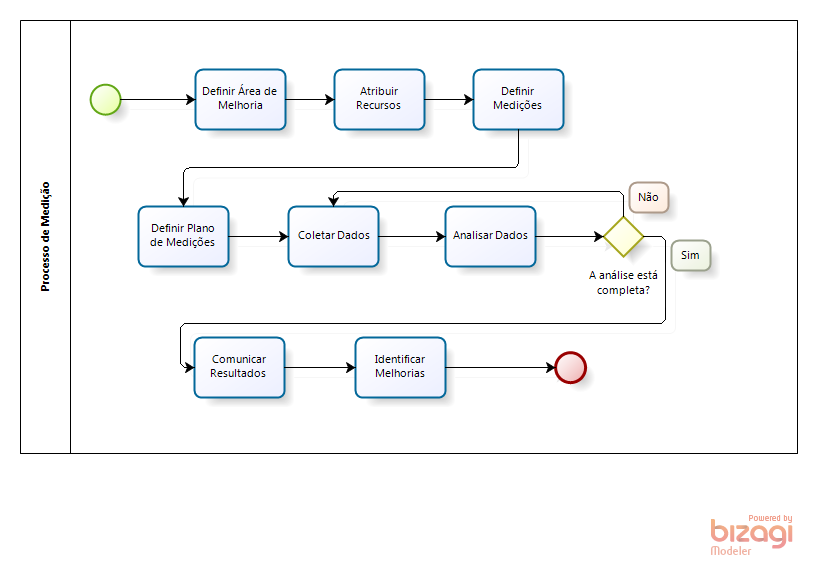
\includegraphics[scale=0.75]{figuras/medicao}
		\label{img:processo}
		\caption{Visão geral do Processo de Medição}
\end{figure}
